%%%%%%%%%%%%%%%%%%%%%%%%%%%%%%%%%%%%%%%
% Header                              %
%%%%%%%%%%%%%%%%%%%%%%%%%%%%%%%%%%%%%%%
% 
% Revisions: 2017-12-12 Martin Raedel <martin.raedel@dlr.de>
%                       Initial draft
%               
% Contact:   Martin Raedel,  martin.raedel@dlr.de
%            DLR Composite Structures and Adaptive Systems
%          
%                                 __/|__
%                                /_/_/_/  
%            www.dlr.de/fa/en      |/ DLR
% 
%%%%%%%%%%%%%%%%%%%%%%%%%%%%%%%%%%%%%%%
% Content                             %
%%%%%%%%%%%%%%%%%%%%%%%%%%%%%%%%%%%%%%%

\begin{tikzpicture}[
  every node/.style={font=\figurefontsize},
  %inner sep=0pt,
]
  % External figure
  \node[anchor=south west,inner sep=0] (image) at (0,0) {
    %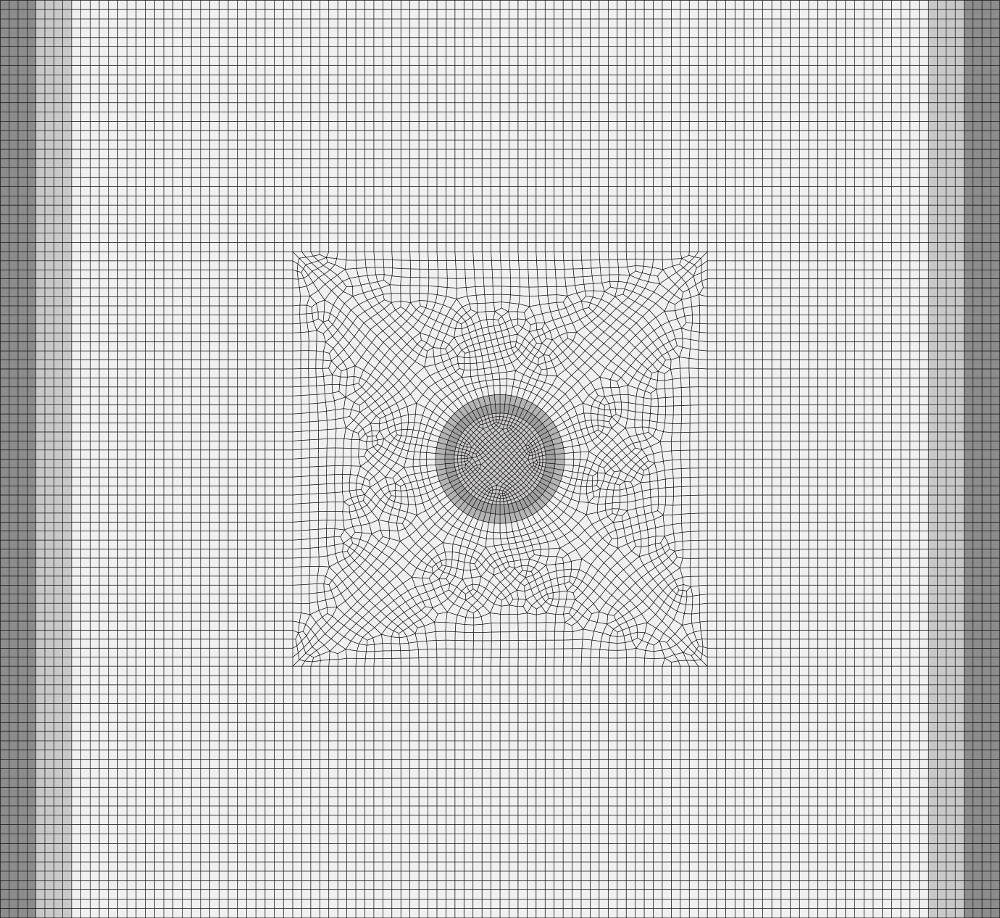
\includegraphics[width=\figwidth,height=\figheight,keepaspectratio]{Model_Fibre_FE_Hex_color_mod_1000}
    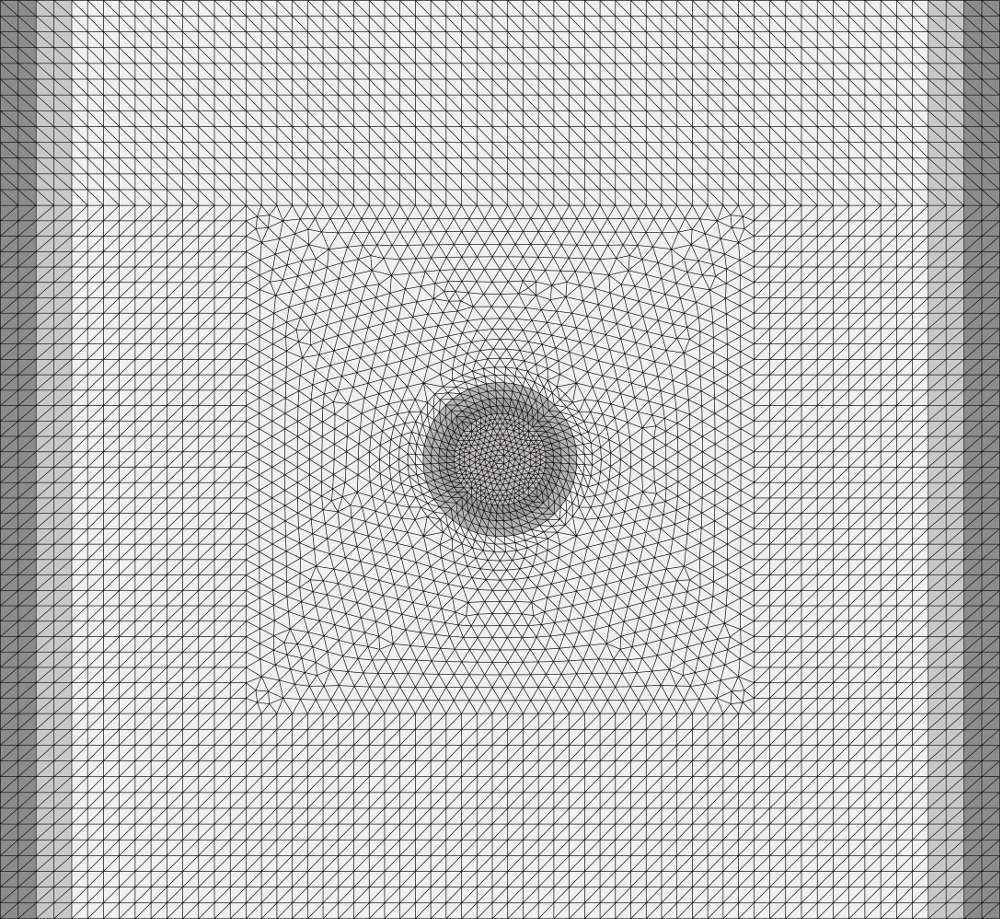
\includegraphics[width=\figwidth,height=\figheight,keepaspectratio]{Model_Fibre_FE_Tet_color_mod_1000}
  };
  % Figure scope
  \begin{scope}[
    x={(image.south east)},
    y={(image.north west)},
  ]
    
    % Load arrows
    \foreach \y in {0,1,...,\numarrows} {\draw[-latex] (-0.025,\y/\numarrows) -- (-0.15,\y/\numarrows) coordinate (loadarrowleft\y);}
    \foreach \y in {0,1,...,\numarrows} {\draw[-latex] ( 1.025,\y/\numarrows) -- ( 1.15,\y/\numarrows) coordinate (loadarrowright\y);}
    
    % Labels
    \node[anchor=south,inner sep=1pt] (matrixndlabel) at (0.5,1.0) {Matrix (no damage)};
    \draw[thin] (matrixndlabel.west) -- (0.06,0.94);
    \draw[thin] (matrixndlabel.east) -- (0.94,0.94);
    
    \node[anchor=south,inner sep=1pt] (lbclabel) at (matrixndlabel.north) {Boundary condition region};
    \draw[thin] (lbclabel.west) -- (0.02,0.98);
    \draw[thin] (lbclabel.east) -- (0.98,0.98);
    
    \node[anchor=north west,inner sep=1pt,yshift=-2pt] (matrixlabel) at (0.1,0) {Matrix};
    \draw[thin] (matrixlabel) -- (0.15,0.25);
    \draw[thin] (matrixlabel) -- (0.455,0.445);
    
    \node[anchor=north east,inner sep=1pt,yshift=-2pt] (fibrelabel) at (0.9,0) {Fibre};
    \draw[thin] (fibrelabel) -- (0.5,0.5);
    \draw[thin] (fibrelabel) -- (0.55,0.5);
    
    % Help grid and labels
    %\pic{myimagegrid};
  \end{scope}
\end{tikzpicture}